\chapter{Become Worthy of Hope}

Hope is not a decoration of life. It is working capital.

A person who has hope can tolerate awkward beginnings, delayed feedback, temporary loneliness, and the long flat part of the compounding curve. A person without hope will sell the future too cheaply, abandon useful skills too early, and mistake other people's mockery for evidence.

But hope is also fragile. It can be extinguished by ridicule, by unreasonable expectations, by public self-display before real results exist, and by the habit of looking for defects in everyone. Therefore, a serious practitioner of wealth freedom has two duties at once:

\begin{enumerate}
\item protect his own hope;
\item stop damaging the hope of others.
\end{enumerate}

The second duty is not merely moral. It is practical. A person who encourages others becomes more welcome in the world, understands long-term growth more deeply, and gradually becomes less dependent on external encouragement. He becomes a source of energy instead of a consumer of it.

\section*{Every Strange Behavior Has a Reason}

Consider a small cultural puzzle. In Western stories, Superman usually flies with his body stretched forward. In many older Chinese stories, immortals fly while standing upright.

One posture looks aerodynamic. The other looks strange to a modern eye. But both are reasonable inside their own mental operating systems. Superman was imagined in a world where air resistance was already a familiar concept. The older immortals were imagined in a world where that concept was not yet installed in ordinary imagination.

The lesson is not about flight. The lesson is that even absurd-looking behavior often has an internal logic.

This matters when you begin to improve yourself. Many people are surprised by what happens next. They expect support and receive mockery. They expect congratulations and receive cold water. They expect family, colleagues, and friends to say, ``Good, keep going,'' but instead hear suspicion, sarcasm, or silence.

At first this seems malicious. Why would anyone attack another person's progress? Does everyone not want to improve? Is progress not a good thing?

The answer is uncomfortable: your progress may make others feel as if they are regressing.

This does not mean you are wrong to improve. It means you must understand the social physics around improvement.

\section*{The Flat Part of Progress}

True progress rarely becomes visible at the beginning. At the starting point, progress is only a wish. Later it becomes a few actions. Only after repeated correct action over a long period does it become visible evidence.

The shape resembles compound growth. For a long time, the curve seems almost flat. Nothing dramatic appears. Then, after enough time and enough accumulation, the line begins to rise in a way that even outsiders can see.

\begin{center}
\begin{adjustbox}{max width=\linewidth}
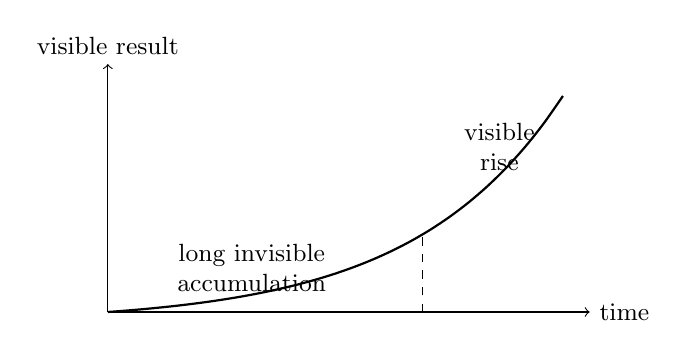
\begin{tikzpicture}[x=0.85cm,y=0.75cm, every node/.style={font=\small}]
\draw[->] (0,0) -- (7.2,0) node[right] {time};
\draw[->] (0,0) -- (0,4.2) node[above] {visible result};
\draw[domain=0:6.8,smooth,variable=\x,thick] plot ({\x},{0.18*exp(0.45*\x)-0.18});
\draw[dashed] (4.7,0) -- (4.7,1.3);
\node[align=center] at (2.15,0.75) {long invisible\\accumulation};
\node[align=center] at (5.85,2.8) {visible\\rise};
\end{tikzpicture}
\end{adjustbox}
\end{center}

The problem is that most people live emotionally on the flat part. They cannot see their own growth clearly. They are tired. They compare themselves with others. They wonder whether yesterday and today are any different. Their own hope is already a small flame.

Then you announce your plan. You say you are learning investing, writing, programming, English, design, sales, public speaking, or a new business skill. Perhaps you say it with excitement. Perhaps you want support. Perhaps you are only reporting the truth.

But to the listener, your unfinished progress may sound like a hidden accusation: ``I am moving; you are not.''

No one likes to be proved backward. No one likes relative regression. No one likes to be made passive in someone else's story of growth. If you feel anxiety when a peer seems to advance while you remain still, then you already understand the mechanism. Others feel it too.

So when people pour cold water on your effort, do not rush to label them bad. Often they are simply uncomfortable. Your hope has touched the wound of their own abandoned hope.

\section*{Spending Future Results Too Early}

There is a deeper mistake.

Before real results exist, public self-proving is a kind of premature spending. You are using a future result, which may or may not occur, to buy present recognition. You are borrowing status from an unearned outcome.

Even if your plan is sincere, the social transaction feels unfair. You have not yet completed the long action. You have not yet paid the full price. You have not yet survived the flat part. Yet you are already asking for the emotional reward of achievement.

This is why many declarations create resistance.

\begin{quote}
A result achieved needs no proof. A result not yet achieved cannot be proved by speech.
\end{quote}

This principle saves attention. If you have not done the work, explaining the future consumes energy that should be used for the work itself. If you have done the work, the result will carry more weight than your explanation.

The practical strategy is simple:

\begin{quote}
Complete the evolution quietly.
\end{quote}

Quietness is not secrecy for its own sake. It is respect for time. It is also respect for other people's fragile hope. Do not demand that others applaud a process whose evidence has not yet arrived.

This does not mean you can never discuss goals. Some goals require coordination, accountability, or explicit partnership. But casual broadcasting is usually expensive. It invites judgment too early, converts a private process into a public performance, and gives the mind a false taste of completion before completion exists.

\section*{Metacognition as Self-Rescue}

When caught inside a problem, it is hard to see the shape of the problem. A person cannot pull himself off the earth by his own hair. In the same way, a mind trapped inside its immediate emotion often cannot escape by more emotion.

This is why metacognition matters.

Metacognition is the ability to stand above one's own thinking and inspect it. It asks, ``What am I assuming? What am I ignoring? What hidden rule is controlling my reaction?'' It turns self-reflection from a slogan into a tool.

When someone mocks your effort, the first reaction may be anger. Metacognition adds a second layer:

\begin{enumerate}
\item What exactly did I say or do?
\item Did I try to obtain recognition before results existed?
\item Did I make the other person feel relatively worse?
\item Is this person's reaction useful information, or merely noise?
\item What adjustment protects both my progress and my peace?
\end{enumerate}

This is not self-blame in the weak sense. It is self-command. If you can locate your own contribution to the friction, you regain freedom to act differently.

A useful practice is to maintain a small mental pop-up list: the traps you fall into repeatedly. For example: explaining too much, showing unfinished plans, arguing with people who have not asked, judging others quickly, and treating temporary discouragement as permanent truth. Review the list often enough, and it gradually becomes part of your operating system.

\section*{A Better Map of the Jungle}

Many people imagine society as a jungle. In that picture, some are weak, some are strong, some hunt, and some hide. The metaphor is partly useful. People do compete. Risks exist. Power matters. Naivete is costly.

But the metaphor is incomplete.

In nature, a rabbit does not become a leopard. In human society, a person can change category. A poor learner can become a strong learner. A low-income worker can become a valuable professional. A person with no capital can slowly accumulate capital. A timid beginner can become someone with works, skills, reputation, and judgment.

The social jungle has evolution inside it.

This changes the emotional meaning of current weakness. If you are weak today, that is not a permanent identity. It is a present condition. You may need to pass through several intermediate stages before the change is obvious, but the possibility exists.

\begin{center}
\begin{adjustbox}{max width=\linewidth}
\begin{tikzpicture}[node distance=0.55cm, every node/.style={font=\small, align=center}]
\node[draw, rounded corners, minimum width=2.1cm, minimum height=0.7cm] (wish) {wish};
\node[draw, rounded corners, minimum width=2.1cm, minimum height=0.7cm, right=of wish] (action) {action};
\node[draw, rounded corners, minimum width=2.1cm, minimum height=0.7cm, right=of action] (repeat) {long\\repetition};
\node[draw, rounded corners, minimum width=2.1cm, minimum height=0.7cm, right=of repeat] (evolve) {evolution};
\draw[->] (wish) -- (action);
\draw[->] (action) -- (repeat);
\draw[->] (repeat) -- (evolve);
\end{tikzpicture}
\end{adjustbox}
\end{center}

This is why the word ``evolution'' is often better than ``improvement.'' Improvement can sound immediate. Evolution carries time inside the word. It reminds you that a real change of species, even in a metaphorical sense, is not a weekend project.

The right conclusion is not, ``I must prove I am no longer weak.'' The right conclusion is, ``I must keep evolving until proof is unnecessary.''

\section*{Becoming Welcome While Still Small}

There remains a practical question: while still weak, how should one live among stronger and weaker people?

One early answer is to become cheerful.

Optimism is often misunderstood as a natural personality trait. In practice, optimism is also a choice and an ability: the chosen ability to believe that tomorrow can be better because correct action today can make it so. It can be strengthened by learning, movement, sleep, useful work, and association with people who still have energy for the future.

A cheerful beginner is easier to help than a bitter beginner. This is not because cheerful people are morally superior. It is because bitterness consumes the attention of everyone nearby. Cheerfulness lowers the cost of being around you.

But cheerfulness is only the first level. A stronger strategy is to become encouraging.

Encouragement is scarce. Cold water is everywhere. Sarcasm is cheap. Advice no one asked for is abundant. Encouragement, especially accurate encouragement, is rare.

To encourage someone is not to flatter him. It is not to pretend his work is good when it is not. Real encouragement protects the person's hope while leaving room for correction. It says, in word or action, ``Continue. This is worth improving. Your current awkwardness is not final.''

Sometimes a plain sentence is enough: ``I support you.'' Sometimes presence is enough. Sometimes the best encouragement is to listen without turning the other person's unfinished effort into a stage for your own cleverness.

\section*{Encouragement as a Compound Asset}

Encouraging others produces two direct returns.

First, people naturally prefer the company of someone who carries a scarce resource. If you consistently protect rather than damage hope, you become easier to trust. This does not require manipulation. It is simply how value works. People move toward what helps them continue.

Second, by encouraging others, you slowly become less dependent on being encouraged yourself. You see many people survive the flat part. You watch small efforts become visible results. You gather evidence that correct action compounds. Eventually the evidence is no longer theoretical. It has passed through the lives of people around you.

Then encouragement becomes self-reinforcing.

\begin{center}
\begin{adjustbox}{max width=\linewidth}
\begin{tikzpicture}[node distance=0.7cm, every node/.style={font=\small, align=center}]
\node[draw, rounded corners, minimum width=2.5cm, minimum height=0.75cm] (give) {encourage\\others};
\node[draw, rounded corners, minimum width=2.5cm, minimum height=0.75cm, right=of give] (see) {observe\\continuation};
\node[draw, rounded corners, minimum width=2.5cm, minimum height=0.75cm, below=of see] (believe) {trust\\compounding};
\node[draw, rounded corners, minimum width=2.5cm, minimum height=0.75cm, left=of believe] (stable) {need less\\external proof};
\draw[->] (give) -- (see);
\draw[->] (see) -- (believe);
\draw[->] (believe) -- (stable);
\draw[->] (stable) -- (give);
\end{tikzpicture}
\end{adjustbox}
\end{center}

This is one of the quiet surprises of practice: by becoming a source of encouragement, you become more stable. You no longer wait helplessly for the world to provide the exact words you need. You have trained yourself to generate them truthfully.

\section*{Three Praises}

Self-reflection is necessary. A person should review errors, correct behavior, and take responsibility. But if reflection becomes only self-criticism, it weakens hope.

A useful supplement is daily self-praise.

Not empty praise. Not vanity. Accurate praise.

At the end of the day, ask:

\begin{enumerate}
\item What did I do correctly today?
\item What difficulty did I overcome?
\item What small action deserves to be repeated tomorrow?
\end{enumerate}

This practice matters because no one else sees the full cost of your effort. Others see the finished sentence, not the resistance before writing it. They see the trade, not the emotional restraint before making it. They see the workout, not the negotiation with laziness before leaving home. They see the calm reply, not the anger you chose not to feed.

You are often the best witness to your own invisible work. If you never acknowledge it, you train yourself to believe that only external applause counts. That is a fragile way to live.

Self-praise and self-criticism should work together:

\begin{center}
\begin{adjustbox}{max width=\linewidth}
\begin{tabular}{p{0.36\linewidth}p{0.5\linewidth}}
\hline
Practice & Function \\
\hline
Reflection & Find errors and repair methods. \\
Self-praise & Preserve evidence that effort is working. \\
Encouraging others & Strengthen a world where hope can survive. \\
Quiet execution & Let real results replace premature proof. \\
\hline
\end{tabular}
\end{adjustbox}
\end{center}

A person who only praises himself becomes blind. A person who only criticizes himself becomes exhausted. The better discipline is to correct what is wrong and reinforce what is right.

\section*{Do Not Be Harsh}

Harshness is easy. Anyone can find defects in anyone. If you decide to be sharp enough, every beginner looks foolish, every attempt looks incomplete, and every hope looks naive.

But harshness is usually a misuse of attention.

To build wealth freedom, attention must be placed on growth, value, capital, execution, and long-term compounding. Spending attention on casual contempt is expensive. It teaches the mind to scan for weakness instead of possibility. Over time, your world becomes uglier because your search function has been trained to find ugliness.

Looking for strengths is not sentimental. It is strategic. Every person's strength is a clue to what keeps that person moving. When you notice it and encourage it, you are helping preserve the small engine of future improvement.

This also makes you a better investor in people. You begin to see not only current output, but possible trajectory. You become less likely to dismiss a beginner because the first version is clumsy. You remember that no one starts with finished excellence.

The phrase ``This is just my personality'' is often an excuse for refusing to evolve. A person says, ``I either do it well or I do not do it.'' It sounds principled, but it hides a false demand: to do well from the beginning. Almost no meaningful skill allows that. If you insist on starting only when you can already perform well, you will never start anything important.

\section*{Works Before Words}

Action is stronger than language by several orders of magnitude.

If you want to help others, first become someone with works. A work may be an article, a product, a business, a portfolio, a record of investment discipline, a useful tool, a trained skill, or a visible body of service. Works reduce the need for self-proclamation. They make advice more credible because they show that the speaker has paid some price.

This is why ``being qualified to say the sentence'' matters. The same sentence has different weight in different mouths. A person who has not acted may speak a correct principle and still be ignored. A person whose life contains evidence may say less and be heard more.

Do not resent this. It is reasonable. Trust needs evidence.

Therefore, the path is not to argue for authority. The path is to accumulate evidence.

\begin{enumerate}
\item Do the work.
\item Keep doing it through the invisible period.
\item Let the work become visible.
\item Speak from the evidence, not from the wish.
\end{enumerate}

When people ask for advice, give it carefully. When they do not ask, be cautious. Unsolicited teaching often feels like status-taking. If your work is strong enough, those who need help will often come closer by themselves.

\section*{A Better Jungle}

Even if you become strong, do not use strength to humiliate the weak.

The world itself is changing. Competition remains, but many opportunities no longer require direct predation. Cooperation, specialization, technology, markets, and networks have made many forms of mutual benefit more attractive than simple conflict. In many cases, attacking others is more costly than building one's own position.

The better strategy is to find a place where you can grow without constantly injuring others. In a world with expanding possibility, wealth freedom is not served by treating every relationship as a zero-sum fight. It is served by increasing value, protecting attention, building capital, and joining or creating arrangements where more than one side can win.

This does not require naivete. Risk still exists. Some people do harm. Boundaries are necessary. But a person who sees only enemies will waste his life in defensive posture. A person who sees possible evolution, in himself and in others, can act with more calm.

The deepest change is this: the world no longer needs to be divided into ``people I like'' and ``people I hate.'' A more useful division is ``people I already like'' and ``people I have not yet learned to like.'' This does not mean trusting everyone. It means refusing to let contempt become the default operating system.

\section*{The Practice}

To become worthy of hope, practice these rules in ordinary life:

\begin{enumerate}
\item Keep unfinished evolution quiet unless speech is necessary for action.
\item Do not use future results to buy present status.
\item When others resist your progress, inspect the social mechanism before judging their character.
\item Replace ``progress'' with ``evolution'' when you need a stronger sense of time.
\item Encourage at least one person every day.
\item Praise yourself accurately for actions worth repeating.
\item Avoid harshness, especially toward beginners.
\item Build works so that your words eventually stand on evidence.
\item If you become strong, do not use strength to damage hope.
\end{enumerate}

None of these practices is dramatic. That is why they work. The future is usually changed by repeated ordinary actions that most people underestimate.

Hope begins as a small flame. Repetition feeds it. Metacognition protects it. Quiet execution gives it material. Encouragement spreads it without reducing it.

A person who understands this becomes easier to help, harder to discourage, and less tempted to injure others on the way forward. He no longer needs to prove every step. He is busy becoming the kind of person whose results will eventually speak clearly enough.
